\documentclass[letter, 10pt]{article}
\usepackage[utf8]{inputenc}
\usepackage[T1]{fontenc}
\usepackage{lmodern}
\usepackage[spanish, es-tabla]{babel}
\usepackage{amsfonts}
\usepackage{amsmath}
\usepackage{amssymb}
\usepackage{graphicx}
\usepackage{url}
\usepackage{booktabs}
\usepackage{multirow}
\usepackage{tikz}
\usetikzlibrary{babel}
\usepackage{array}
\usepackage[font=small]{caption}
\usepackage[ruled,vlined,linesnumbered,spanish]{algorithm2e}
\usepackage[top=3cm,bottom=3cm,left=3.5cm,right=3.5cm,footskip=1.5cm,headheight=1.5cm,headsep=.5cm,textheight=3cm]{geometry}

% Separacion entre figuras/tablas y texto
\setlength{\textfloatsep}{10pt plus 2pt minus 2pt}
\setlength{\floatsep}{8pt plus 2pt minus 2pt}
\setlength{\intextsep}{8pt plus 2pt minus 2pt}
% Espacio vertical de las ecuaciones
\AtBeginDocument{\setlength{\abovedisplayskip}{6pt plus 2pt minus 2pt}\setlength{\belowdisplayskip}{6pt plus 2pt minus 2pt}\setlength{\abovedisplayshortskip}{3pt plus 2pt}\setlength{\belowdisplayshortskip}{4pt plus 2pt minus 2pt}}
\renewcommand{\topfraction}{0.9}\renewcommand{\bottomfraction}{0.8}
\renewcommand{\textfraction}{0.07}\renewcommand{\floatpagefraction}{0.85}
\setcounter{topnumber}{3}\setcounter{bottomnumber}{2}\setcounter{totalnumber}{5}
% Palabras clave del pseudocodigo en espanol
\SetKwInput{KwIn}{Entrada}\SetKwFor{While}{mientras}{hacer}{fin}\SetKwFor{ForEach}{para cada}{hacer}{fin}
\SetKwIF{If}{ElseIf}{Else}{si}{entonces}{si no, si}{si no}{fin}\SetKw{Return}{devolver}
% Inserta filas de tabla generadas por experimentos/analizar.py (compatible con booktabs)
\makeatletter\newcommand{\filastabla}[1]{\@@input #1 }\makeatother

\begin{document}
\title{Inteligencia Artificial \\ \begin{Large}Informe Final: Generaci\'on de Niveles de Plataformas\end{Large}}
\author{Agust\'in Venegas Fellenberg -- 202273104-4}
\date{20 de noviembre de 2026}
\maketitle

%--------------------No borrar esta secci\'on--------------------------------%
\section*{Evaluaci\'on}

\begin{tabular}{ll}
C\'odigo Fuente (20 \%): & \underline{\hspace{2cm}}\\
Resumen (2 \%): & \underline{\hspace{2cm}}\\
Introducci\'on (3 \%): & \underline{\hspace{2cm}}\\
Representaci\'on (10 \%): & \underline{\hspace{2cm}} \\
Descripci\'on del algoritmo (20 \%): & \underline{\hspace{2cm}} \\
Experimentos (10 \%): & \underline{\hspace{2cm}} \\
Resultados (10 \%): & \underline{\hspace{2cm}} \\
Conclusiones (20 \%): & \underline{\hspace{2cm}}\\
Bibliograf\'ia (5 \%): & \underline{\hspace{2cm}}\\
 & \\
\textbf{Nota Final (100 \%)}: & \underline{\hspace{2cm}}
\end{tabular}
%---------------------------------------------------------------------------%

\begin{abstract}
El dise\~no manual de niveles de videojuegos es costoso, y la Generaci\'on Procedural de Contenido (PCG) lo automatiza mediante algoritmos. Este informe estudia la generaci\'on de niveles de plataformas 2D completables, coherentes con la f\'isica del personaje, con la cantidad solicitada de plataformas, enemigos y obst\'aculos y con la linealidad pedida. Se revisa la literatura del \'area, se formula un modelo de Programaci\'on con Restricciones y se implementa en C++ un algoritmo evolutivo sobre una representaci\'on por columnas, con un modelo de salto que discretiza la par\'abola del salto por columnas y operadores que act\'uan sobre tramos del nivel. En seis instancias de prueba, el algoritmo obtiene niveles completables con las cantidades exactas en las 180 ejecuciones, en promedio en 1,1~s, con alturas variadas entre semillas.
\end{abstract}

%=============================================================================
\section{Introducci\'on}
%=============================================================================
La industria de los videojuegos ha experimentado un crecimiento sostenido, lo que ha aumentado la competencia entre estudios y las expectativas de los jugadores respecto de la cantidad y calidad del contenido~\cite{DePontes2022, Saavedra2026}. Producir ese contenido manualmente es costoso: el desarrollo de un juego de alto presupuesto puede extenderse entre uno y tres a\~nos e involucrar a cientos de profesionales~\cite{DePontes2022}. A ello se suma la valoraci\'on de la rejugabilidad, es decir, el inter\'es del jugador por volver a jugar un mismo juego, que aumenta cuando cada partida ofrece un escenario distinto~\cite{DePontes2022, Smith2011}, aspecto especialmente importante en el g\'enero \emph{Roguelike}~\cite{Saavedra2026}. La Generaci\'on Procedural de Contenido (PCG), definida como la creaci\'on de contenido de juego mediante algoritmos~\cite{Togelius2011}, responde a estas necesidades y constituye la motivaci\'on de este trabajo.

El problema abordado consiste en generar autom\'aticamente un nivel de plataformas, al estilo de \emph{Super Mario Bros.} (1985), que sea completable, que ubique correctamente sus elementos y cuya cantidad de plataformas, enemigos y obst\'aculos sea lo m\'as cercana posible a la solicitada~\cite{Saavedra2026}.

El prop\'osito de este informe es presentar el estudio completo del problema: su estado del arte, un modelo matem\'atico y la implementaci\'on y evaluaci\'on de un algoritmo evolutivo (AE) que lo resuelve. Sus contribuciones son un modelo de Programaci\'on con Restricciones que expresa la completitud como un flujo, un modelo de salto que discretiza la par\'abola por columnas y permite derrotar enemigos y un AE con operadores por tramos. Los experimentos, con seis instancias de prueba y 30 semillas, muestran que el AE obtiene niveles completables con las cantidades exactas en las 180 ejecuciones, en promedio en 1,1~s. Las Secciones~\ref{sec:def} a~\ref{sec:modelo} presentan el problema, su estado del arte y el modelo; las Secciones~\ref{sec:rep} y~\ref{sec:alg}, la representaci\'on y el algoritmo, incluida la respuesta al Estado de Avance; las Secciones~\ref{sec:exp} y~\ref{sec:res}, los experimentos y resultados, y la Secci\'on~\ref{sec:conc}, las conclusiones.

\section{Definici\'on del Problema}
\label{sec:def}

El problema consiste en crear autom\'aticamente un nivel bidimensional que un personaje debe recorrer desde un punto de inicio hasta una meta. Para avanzar, el personaje camina y salta sobre plataformas mientras evita enemigos, obst\'aculos y ca\'idas al vac\'io~\cite{Compton2006, Saavedra2026}.

Las variables del problema describen la construcci\'on del nivel. Para cada plataforma se decide si se utiliza, d\'onde comienza, a qu\'e altura se ubica y cu\'al es su largo. Para cada enemigo y obst\'aculo se decide si aparece en el nivel y, en tal caso, sobre qu\'e plataforma y en qu\'e posici\'on. Estas decisiones admiten distintas representaciones: celda por celda en una grilla, por columnas completas, por segmentos predise\~nados o mediante par\'ametros generales que luego se transforman en el nivel~\cite{Togelius2011, Dahlskog2013, DePontes2022}.

Las restricciones son de dos tipos. Las geom\'etricas exigen que las plataformas queden dentro del nivel, respeten un tama\~no permitido y no se superpongan; que cada enemigo u obst\'aculo se ubique sobre una plataforma, y que el inicio y el final del nivel est\'en definidos~\cite{Saavedra2026}. La restricci\'on de completitud exige que exista una secuencia de saltos factibles para el personaje que conecte el inicio con la meta. Esta depende del alcance del salto y es la m\'as dif\'icil de verificar, pues involucra la relaci\'on entre todas las plataformas~\cite{Compton2006, Smith2011}.

El objetivo principal es que la cantidad de plataformas, enemigos y obst\'aculos del nivel sea lo m\'as cercana posible a la solicitada~\cite{Saavedra2026}. Adem\'as, se consideran la est\'etica, la variedad entre niveles generados, la densidad de enemigos y obst\'aculos, y la linealidad del recorrido~\cite{Saavedra2026}, esta \'ultima entendida como el grado en que las alturas de las plataformas se ajustan a una recta~\cite{Smith2011}.

El problema presenta varias dificultades. En primer lugar, el espacio de niveles es muy grande y solo una regi\'on peque\~na corresponde a niveles jugables~\cite{Dahlskog2013}; la Secci\'on~\ref{sec:espacio} muestra que crece exponencialmente con la cantidad de elementos. En segundo lugar, verificar la completitud suele requerir simular la f\'isica del personaje o un agente, lo que encarece cada evaluaci\'on~\cite{Green2020,DePontes2022}. En tercer lugar, los criterios pueden entrar en conflicto: por ejemplo, solicitar muchos enemigos y obst\'aculos con pocas plataformas obliga a concentrarlos, lo que aumenta la densidad y puede impedir que el nivel sea completable; de forma an\'aloga, Smith et al.~\cite{Smith2011} observan que ciertas combinaciones de componentes no pueden ajustarse a la forma deseada del nivel. Por \'ultimo, cualidades como la diversi\'on o el ritmo son dif\'iciles de formalizar en una m\'etrica~\cite{Togelius2011, Dahlskog2013}.


En cuanto a las variantes, una primera distinci\'on es entre generaci\'on \emph{offline} y \emph{online}. En la generaci\'on offline el nivel se crea antes de jugarse, lo que admite un alto costo computacional, como las 10.000 generaciones del algoritmo evolutivo de Dahlskog y Togelius~\cite{Dahlskog2013}. En la generaci\'on online el nivel se crea durante el juego; el caso extremo son los juegos infinitos, donde cada tramo debe generarse antes de que el jugador termine el anterior~\cite{Togelius2011, DePontes2022}. Una segunda distinci\'on es entre niveles de camino \'unico y niveles con m\'ultiples caminos, que incluyen bifurcaciones, caminos paralelos, retrocesos y portales~\cite{Compton2006}; esta distinci\'on se refiere a la estructura del recorrido y no a la linealidad de las alturas definida anteriormente. Otras variantes adaptan el nivel a un jugador~\cite{Togelius2011}, imitan el estilo de un juego existente~\cite{Dahlskog2013, Summerville2016} o parten de una secuencia de mec\'anicas que el jugador debe ejecutar~\cite{Green2020}. La variante estudiada consiste en generar un nivel cuyas cantidades de plataformas, enemigos y obst\'aculos se acerquen lo m\'as posible a las solicitadas, respetando las restricciones geom\'etricas y de completitud descritas~\cite{Saavedra2026}.


\section{Estado del Arte}
\label{sec:ea}

El uso de PCG en videojuegos se remonta a fines de la d\'ecada de 1970: \emph{Beneath Apple Manor} (1978) es el uso m\'as antiguo conocido~\cite{Summerville2016}, seguido por \emph{Rogue} y \emph{Akalabeth} en 1980~\cite{DePontes2022}. Inicialmente se emple\'o para superar limitaciones de memoria; \emph{Elite} (1984), por ejemplo, almacenaba galaxias completas mediante un algoritmo determinista a partir de una semilla~\cite{Togelius2011, DePontes2022}. Sin embargo, a mediados de la d\'ecada de 2000 a\'un no exist\'ian juegos de plataformas comerciales con niveles generados, porque en este g\'enero peque\~nas variaciones pueden volver imposible un nivel~\cite{Compton2006}. En el \'ambito acad\'emico, Compton y Mateas~\cite{Compton2006} propusieron en 2006 un modelo jer\'arquico de niveles de plataformas, que Smith et al.~\cite{Smith2011} identifican como el trabajo previo dedicado espec\'ificamente a este g\'enero. Posteriormente, Togelius et al.~\cite{Togelius2011} propusieron una taxonom\'ia de la PCG basada en b\'usqueda.

\subsection{M\'etodos empleados}

Togelius et al.~\cite{Togelius2011} distinguen los m\'etodos \emph{constructivos}, que generan el contenido en una sola pasada usando solo operaciones que preservan su validez, de los de \emph{generar y probar}, que producen candidatos y luego los verifican; entre estos \'ultimos se encuentran los basados en b\'usqueda, donde una funci\'on de evaluaci\'on gu\'ia a una metaheur\'istica. Adem\'as, los niveles son contenido \emph{necesario}, por lo que un nivel no jugable es inaceptable, y su evaluaci\'on puede ser directa, basada en simulaci\'on o interactiva~\cite{Togelius2011}. Los trabajos revisados se agrupan en cuatro enfoques.

\textbf{Modelos jer\'arquicos.} Compton y Mateas~\cite{Compton2006} dividen un nivel en cuatro capas inspiradas en la representaci\'on del ritmo musical: \emph{componentes} (plataformas, lianas, pinchos), \emph{patrones} que los agrupan en secuencias r\'itmicas, \emph{celdas} que encapsulan patrones y \emph{estructuras de celdas} que introducen bifurcaciones, caminos paralelos y portales. Cada patr\'on se construye con un modelo f\'isico que simula el movimiento del avatar y estima la dificultad de cada salto a partir de la ventana de tiempo de que dispone el jugador para corregirlo en el aire, considerando su precisi\'on y sus reflejos. Un algoritmo de \emph{hill climbing} ajusta los par\'ametros de los componentes, como su posici\'on y tama\~no, hacia la dificultad deseada; los autores observan que el gr\'afico de la funci\'on de evaluaci\'on (la cercan\'ia a la dificultad deseada en funci\'on de esos par\'ametros) es suave y tiene pocos \'optimos locales, por lo que este m\'etodo tiene buenas probabilidades de encontrar el \'optimo. Su ventaja es que estructura el nivel en torno al ritmo y la conectividad; sus limitaciones, que al publicarse solo el constructor de patrones estaba implementado y que no presenta evaluaci\'on experimental~\cite{Compton2006}.

\textbf{Gram\'aticas basadas en ritmo.} Launchpad~\cite{Smith2011} opera en dos niveles. Primero genera un ritmo, es decir, una secuencia temporal de acciones del jugador (moverse y saltar, donde los intervalos sin movimiento se interpretan como esperas). Luego, una gram\'atica traduce cada acci\'on en geometr\'ia (plataformas, abismos, enemigos, resortes, \emph{stompers} y plataformas m\'oviles) que respeta un modelo f\'isico, lo que garantiza que todos los niveles sean jugables. Cada ritmo origina un \emph{grupo r\'itmico}, y los grupos se unen mediante plataformas de descanso. Como la gram\'atica sobregenera, unos \emph{cr\'iticos} seleccionan el mejor candidato (en los ejemplos reportados, entre 1.000) seg\'un su distancia a una l\'inea de control, es decir, una l\'inea que el dise\~nador traza antes de la generaci\'on para indicar la forma que debe seguir el nivel, y seg\'un la similitud de la frecuencia de componentes con la deseada; por ello, seg\'un la taxonom\'ia de Togelius et al.~\cite{Togelius2011}, el m\'etodo combina una generaci\'on constructiva de cada grupo con una selecci\'on de tipo generar y probar. Su an\'alisis de rango expresivo, basado en las m\'etricas de linealidad y leniencia (cu\'an indulgente es el nivel con los errores del jugador)~\cite{Smith2011}, usadas para evaluar generadores de plataformas desde 2010~\cite{Summerville2016}, revel\'o sesgos no intencionados, como un exceso de \emph{stompers} y de escaleras ascendentes. Su ventaja es la jugabilidad garantizada; sus limitaciones, que el control sobre la cantidad de elementos es solo aproximado y que no genera niveles con m\'ultiples caminos~\cite{Smith2011}.

\textbf{Algoritmos evolutivos y de enjambre.} Dahlskog y Togelius~\cite{Dahlskog2013} usan patrones de dise\~no como objetivo de la b\'usqueda y no como piezas de construcci\'on. Cada nivel es una cadena de 200 \emph{cortes verticales} sobre un alfabeto de 24 columnas extra\'idas de \emph{Super Mario Bros.}, evolucionada durante 10.000 generaciones con una estrategia evolutiva $(\mu+\lambda)$, en la que $\mu$ padres generan $\lambda$ hijos por mutaci\'on y los $\mu$ mejores entre padres e hijos forman la siguiente generaci\'on. La funci\'on de evaluaci\'on premia los patrones conocidos y asigna un valor muy negativo, aunque finito, a las secciones no jugables. En un estudio con 24 jugadores, estos niveles resultaron levemente m\'as entretenidos que dos alternativas, con diferencias marginales y sin pruebas estad\'isticas reportadas. Adem\'as, tienden a sobrecargarse y carecer de pausas, y ajustar su funci\'on de evaluaci\'on es complejo~\cite{Dahlskog2013}.

Green et al.~\cite{Green2020} aplican FI-2Pop, un tipo de algoritmo evolutivo que mantiene una poblaci\'on factible y otra infactible, para unir escenas de un corpus de 1.691 escenas generadas previamente con \emph{Constrained MAP-Elites}, un algoritmo evolutivo que, en lugar de una \'unica mejor soluci\'on, conserva la mejor escena para cada combinaci\'on de mec\'anicas, separando las factibles de las infactibles. En FI-2Pop, la poblaci\'on infactible busca niveles completables por un agente A* y la factible, niveles cuyas mec\'anicas coincidan con una secuencia objetivo. Sus niveles alcanzan entre 87,25\% y 100\% de jugabilidad, frente a 25--28,5\% de un generador voraz y 10,75\% de uno aleatorio, aunque son m\'as planos y menos variados que los originales. Cabe notar que el mismo agente completa solo el 52\% de los niveles originales, lo que evidencia los l\'imites de verificar la completitud mediante un agente~\cite{Green2020}.

De Pontes et al.~\cite{DePontes2022} aplican optimizaci\'on por enjambre de part\'iculas (PSO), en la que cada soluci\'on candidata, o part\'icula, se desplaza por el espacio de b\'usqueda atra\'ida por su mejor posici\'on hist\'orica y por la mejor del enjambre, a un juego de plataformas infinito, donde el nivel es una lista de columnas y cada tramo de 100 columnas se genera mientras el jugador avanza. La funci\'on de evaluaci\'on penaliza, entre otros, pinchos contiguos imposibles de sortear y abismos m\'as anchos que el alcance del salto. PSO converge en 10 a 50 iteraciones a mejores soluciones que un algoritmo gen\'etico, que requiere cientos de generaciones; aunque cada iteraci\'on es m\'as costosa, tarda unos 0,6~s frente a unos 4~s del GA, bajo los 12,8~s que, como m\'inimo, el jugador demora en recorrer el tramo. Ninguno garantiza la jugabilidad~\cite{DePontes2022}.

\textbf{Redes neuronales.} Otra alternativa es aprender a generar niveles a partir de ejemplos humanos. Summerville y Mateas~\cite{Summerville2016} se\~nalan que las cadenas de Markov previas carec\'ian de coherencia global y entrenan redes LSTM con 39 niveles (15 de \emph{Super Mario Bros.} y 24 de su secuela japonesa) representados como texto. Con su mejor configuraci\'on, que recorre el nivel en orden serpenteante e incluye la trayectoria del jugador y la profundidad de cada columna, el 97\% de los niveles resulta completable por un agente, m\'as que el mejor m\'etodo previo basado en aprendizaje (66\%) y que el mejor generador de la competencia Mario AI de 2011 (94\%)~\cite{Summerville2016}. Se observa, adem\'as, que el m\'etodo depende de un corpus peque\~no y no permite controlar directamente el contenido del nivel.

\subsection{Representaciones}

Togelius et al.~\cite{Togelius2011} distinguen representaciones directas, donde cada parte del genotipo corresponde a una parte del nivel, de indirectas, que lo describen mediante par\'ametros o reglas que un generador transforma en el nivel, como el ritmo de Launchpad, que una gram\'atica traduce en geometr\'ia~\cite{Smith2011}, y recomiendan representaciones de alta \emph{localidad}, en las que un cambio peque\~no en el genotipo produce un cambio peque\~no en el nivel. Una representaci\'on directa t\'ipica es la matriz de \emph{tiles}, que asigna un tipo de celda (vac\'io, bloque, enemigo, etc.) a cada posici\'on de la grilla; describe cualquier nivel, pero genera un espacio enorme y casi enteramente no jugable, por lo que Dahlskog y Togelius~\cite{Dahlskog2013} la descartaron. Las representaciones por columnas, como los cortes verticales~\cite{Dahlskog2013} y la lista de columnas~\cite{DePontes2022}, reducen el espacio, mientras que las escenas~\cite{Green2020} y los grupos r\'itmicos~\cite{Smith2011} parten de piezas cuya validez ya se conoce. La evidencia cuantitativa m\'as directa sobre el efecto de la representaci\'on proviene de Summerville y Mateas~\cite{Summerville2016}: con la misma red, incluir la trayectoria del jugador eleva la proporci\'on de niveles completables de 67\% a 96\% con el orden de abajo hacia arriba, y de 39\% a 93\% con el orden serpenteante. Es decir, las representaciones m\'as efectivas son las que incorporan informaci\'on sobre c\'omo se recorre el nivel, y no solo sobre su geometr\'ia.

\subsection{S\'intesis comparativa}

La Tabla~\ref{tab:comp} resume los trabajos revisados que generan niveles completos.

\begin{table}[htbp]
\centering
\scriptsize
\begin{tabular}{|p{1.9cm}|p{2.0cm}|p{2.2cm}|p{1.9cm}|p{1.5cm}|p{2.3cm}|}
\hline
\raggedright \textbf{Referencia} & \raggedright \textbf{Enfoque} & \raggedright \textbf{Representaci\'on} & \raggedright \textbf{?`Garantiza jugabilidad?} & \raggedright \textbf{Generaci\'on} & \raggedright \textbf{Resultado principal} \tabularnewline
\hline
\raggedright Compton y Mateas (2006)~\cite{Compton2006} & \raggedright Modelo jer\'arquico y \emph{hill climbing} & \raggedright Componentes, patrones y celdas & \raggedright Parcial (dificultad por patr\'on) & \raggedright Online (propuesta) & \raggedright Sin evaluaci\'on experimental \tabularnewline
\hline
\raggedright Smith et al. (2011)~\cite{Smith2011} & \raggedright Gram\'atica y cr\'iticos (h\'ibrido) & \raggedright Ritmos y grupos r\'itmicos & \raggedright S\'i, por construcci\'on & \raggedright Offline & \raggedright An\'alisis de rango expresivo; sesgos detectados \tabularnewline
\hline
\raggedright Dahlskog y Togelius (2013)~\cite{Dahlskog2013} & \raggedright Estrategia evolutiva & \raggedright 200 cortes verticales (24 s\'imbolos) & \raggedright No (penalizaci\'on) & \raggedright Offline & \raggedright Mejora leve percibida (24 jugadores) \tabularnewline
\hline
\raggedright Summerville y Mateas (2016)~\cite{Summerville2016} & \raggedright Redes LSTM & \raggedright Secuencia de \emph{tiles} con trayectoria & \raggedright No & \raggedright Offline & \raggedright 97\% completables (agente) \tabularnewline
\hline
\raggedright Green et al. (2020)~\cite{Green2020} & \raggedright FI-2Pop sobre escenas & \raggedright Secuencia de escenas & \raggedright No (restricci\'on v\'ia agente A*) & \raggedright Offline & \raggedright 87--100\% jugables (voraz: 25--28,5\%) \tabularnewline
\hline
\raggedright De Pontes et al. (2022)~\cite{DePontes2022} & \raggedright PSO comparado con GA & \raggedright Lista de columnas & \raggedright No & \raggedright Online (infinito) & \raggedright Converge en 10--50 iteraciones (0,6~s) \tabularnewline
\hline
\end{tabular}
\caption{Comparaci\'on de los enfoques revisados.}
\label{tab:comp}
\end{table}

No existe un algoritmo dominante, y los resultados no son directamente comparables, pues cada trabajo emplea juegos, agentes y m\'etricas distintos. Launchpad~\cite{Smith2011} es el \'unico que garantiza jugabilidad por construcci\'on; sin garant\'ia formal, FI-2Pop y las LSTM con trayectoria alcanzan las mayores tasas de completitud medidas con agentes~\cite{Green2020,Summerville2016}, y en generaci\'on online PSO supera en rapidez a un GA~\cite{DePontes2022}. Se repite un mismo compromiso: los m\'etodos que garantizan jugabilidad controlan menos el contenido, y los que ofrecen control y rapidez no la garantizan.

\subsection{Tendencia actual}

La investigaci\'on reciente sigue tres l\'ineas: descomponer el problema en piezas peque\~nas que luego se combinan mediante b\'usqueda~\cite{Green2020,DePontes2022}; incorporar informaci\'on del jugador, como trayectorias o secuencias de mec\'anicas~\cite{Summerville2016, Green2020}, y combinar aprendizaje profundo con b\'usqueda. De Pontes et al.~\cite{DePontes2022} proponen como trabajo futuro integrar redes profundas con optimizaci\'on. Persisten como problemas abiertos la falta de garant\'ias de jugabilidad en los m\'etodos r\'apidos o aprendidos~\cite{DePontes2022, Summerville2016} y la dificultad de medir cualidades como el ritmo~\cite{Dahlskog2013}. Para el aprendizaje autom\'atico en PCG, v\'ease~\cite{Summerville2018}; para el \'area en general,~\cite{Shaker2016}.

\section{Modelo Matem\'atico}
\label{sec:modelo}

\subsection{Paradigma de modelado}

El problema se formula como un \textbf{problema de optimizaci\'on con restricciones} en el paradigma de \textbf{Programaci\'on con Restricciones} (CP). Las variables son enteras y acotadas (posiciones, alturas y largos), y varias restricciones son implicaciones l\'ogicas del tipo ``si el enemigo existe, entonces est\'a sobre una plataforma'', que CP expresa directamente, mientras que la Programaci\'on Lineal Entera Mixta requerir\'ia linealizarlas con constantes Big-M y variables adicionales. La funci\'on objetivo y las restricciones provienen de la definici\'on del problema~\cite{Saavedra2026}; la alcanzabilidad se basa en los modelos f\'isicos del salto de Compton y Mateas~\cite{Compton2006}, Launchpad~\cite{Smith2011} y De Pontes et al.~\cite{DePontes2022}, y la completitud se formula como un problema de flujo en un grafo.

\subsection{Conjuntos y par\'ametros}

Se definen los conjuntos de plataformas candidatas $\mathcal{P} = \{1,\dots,\bar{P}\}$, donde por convenci\'on la plataforma $1$ es el inicio y la $2$ la meta; de enemigos $\mathcal{E} = \{1,\dots,\bar{E}\}$ y de obst\'aculos $\mathcal{O} = \{1,\dots,\bar{O}\}$ candidatos; de columnas $\mathcal{X} = \{0,\dots,W-1\}$, y de filas v\'alidas para una plataforma $\mathcal{Y} = \{1,\dots,H\}$, numeradas de abajo hacia arriba, donde la fila $0$ es el vac\'io inferior; como una entidad ocupa la celda sobre su plataforma, solo puede ubicarse sobre plataformas de las filas $1$ a $H-1$.

Los par\'ametros que definen una instancia son:
\begin{itemize}\setlength{\itemsep}{0pt}\setlength{\parskip}{0pt}
\item $W, H \in \mathbb{Z}^+$: ancho y alto del nivel, medidos en \emph{tiles}.
\item $P^*, E^*, O^* \in \mathbb{Z}_{\geq 0}$: cantidad solicitada de plataformas (incluidas inicio y meta), enemigos y obst\'aculos; $\bar{P} \geq \max(P^*, 2)$, $\bar{E} \geq E^*$, $\bar{O} \geq O^*$: m\'aximos disponibles.
\item $\ell_{\min}, \ell_{\max}$: largo m\'inimo y m\'aximo de una plataforma; $\theta$: separaci\'on horizontal m\'inima entre plataformas que comparten franja vertical.
\item $h_{av}$: altura del avatar; $h_{\max}$: altura m\'axima que gana en un salto; $\lambda \geq 1$: ancho m\'inimo de una zona segura de aterrizaje (al menos el ancho del avatar), todos en \emph{tiles}.
\item $D(\Delta y)$: desplazamiento horizontal m\'aximo entre la columna de despegue y la de aterrizaje cuando la plataforma de destino est\'a $\Delta y$ filas por encima ($\Delta y > 0$) o por debajo ($\Delta y < 0$) de la de origen. Es no creciente en $\Delta y$ y se obtiene del modelo f\'isico del juego~\cite{Compton2006, DePontes2022}.
\item $\delta_{\max} \in (0,1)$: fracci\'on m\'axima de una plataforma ocupada por entidades; $\kappa \geq 1$: m\'aximo de columnas ocupadas consecutivas que el avatar sortea con un salto; $\zeta \geq 0$: cantidad de columnas iniciales sin entidades.
\item $\alpha_P, \alpha_E, \alpha_O > 0$: pesos de la funci\'on objetivo; $\mu \in \{+1,-1\}$: sentido de la linealidad pedido ($+1$ maximizar, $-1$ minimizar); $\beta \geq 0$: peso de la linealidad.
\end{itemize}

\subsection{Variables}

\textbf{Plataformas.} Para cada $i \in \mathcal{P}$: $a_i \in \{0,1\}$ vale 1 si la plataforma $i$ forma parte del nivel; $x_i \in \mathcal{X}$ es la columna de su extremo izquierdo; $y_i \in \mathcal{Y}$, la fila en que se ubica, y $\ell_i \in \{\ell_{\min},\dots,\ell_{\max}\}$, su largo.

\textbf{Enemigos.} Para cada $j \in \mathcal{E}$: $b_j \in \{0,1\}$ vale 1 si el enemigo $j$ est\'a presente; $\pi_j \in \mathcal{P}$ es la plataforma sobre la que se ubica, y $u_j \in \mathcal{X}$, su columna. Su celda resultante es $(u_j,\, y_{\pi_j}+1)$.

\textbf{Obst\'aculos.} Para cada $k \in \mathcal{O}$: $c_k \in \{0,1\}$ vale 1 si el obst\'aculo $k$ est\'a presente; $\sigma_k \in \mathcal{P}$ es su plataforma y $w_k \in \mathcal{X}$, su columna.

\textbf{Alcanzabilidad y camino.} Para cada par ordenado $(i,i') \in \mathcal{P}\times\mathcal{P}$ con $i \neq i'$: $r_{ii'} \in \{0,1\}$ vale 1 si desde la plataforma $i$ es posible saltar a la plataforma $i'$, y $z_{ii'} \in \{0,1\}$ vale 1 si ese salto forma parte del camino escogido entre el inicio y la meta.

Adem\'as, se usan expresiones auxiliares. La cantidad de elementos de cada tipo en el nivel es
\[
N_P = \sum_{i\in\mathcal{P}} a_i, \qquad N_E = \sum_{j\in\mathcal{E}} b_j, \qquad N_O = \sum_{k\in\mathcal{O}} c_k.
\]
Sea $L_i = \{x_i,\dots,x_i+\ell_i-1\}$ el conjunto de columnas de la plataforma $i$. La columna $x$ de la plataforma $i$ est\'a ocupada ($o_{ix}=1$) si contiene un enemigo u obst\'aculo:
\[
o_{ix} = 1 \iff \big(\exists j \in \mathcal{E}: b_j = 1 \wedge \pi_j = i \wedge u_j = x\big) \,\vee\, \big(\exists k \in \mathcal{O}: c_k = 1 \wedge \sigma_k = i \wedge w_k = x\big).
\]
Con esto se definen $T_i$, las columnas libres de la plataforma $i$ desde donde se puede saltar,
\[
T_i = \{\, x \in L_i : o_{ix} = 0 \,\},
\]
y $Z_{i'}$, las zonas libres de ancho $\lambda$ donde se puede aterrizar en la plataforma $i'$, identificadas por su primera columna:
\[
Z_{i'} = \{\, x' : \{x',\dots,x'+\lambda-1\} \subseteq L_{i'},\;\; o_{i'x''} = 0 \;\; \forall x'' \in \{x',\dots,x'+\lambda-1\} \,\}.
\]
Por \'ultimo, la distancia horizontal entre una columna de despegue $x$ y una zona de aterrizaje que comienza en $x'$ es $\eta(x,x') = \max\{0,\; x' - x,\; x - (x'+\lambda-1)\}$, y la linealidad del nivel, medida como en Launchpad~\cite{Smith2011}, es la desviaci\'on vertical media de las columnas con plataforma respecto de la recta $\hat{y}(x) = mx + n$ ajustada por m\'inimos cuadrados a esos puntos:
\[
\Lambda = \frac{1}{|C|}\sum_{x\in C} \left| y(x) - \hat{y}(x) \right|, \qquad C = \{x \in \mathcal{X} : \exists i,\; a_i = 1 \wedge x \in L_i\},
\]
donde $y(x)$ es la fila de la plataforma que ocupa la columna $x$. Un valor bajo de $\Lambda$ corresponde a un nivel lineal.

\subsection{Funci\'on objetivo}

\begin{equation}
\min\; F = \underbrace{\alpha_P\,\left|N_P - P^*\right| + \alpha_E\,\left|N_E - E^*\right| + \alpha_O\,\left|N_O - O^*\right|}_{f} \;+\; \beta\,\mu\,\Lambda
\end{equation}

Es decir, se busca el nivel v\'alido cuyas cantidades sean lo m\'as cercanas posible a las solicitadas y, entre ellos, el de linealidad m\'as alta (si $\mu = +1$, se minimiza $\Lambda$) o m\'as baja (si $\mu = -1$, se maximiza $\Lambda$). Con $\alpha_P = \alpha_E = \alpha_O = 1$, $f$ es la funci\'on propuesta en la definici\'on del problema, $f = \Delta_{\text{platforms}} + \Delta_{\text{enemies}} + \Delta_{\text{obstacles}}$~\cite{Saavedra2026}, cuyo \'optimo ideal es $f = 0$. Los pesos permiten priorizar un tipo de elemento cuando las cantidades no pueden satisfacerse simult\'aneamente, por ejemplo, cuando la densidad m\'axima impide ubicar todos los enemigos solicitados. Para que la linealidad sea un criterio secundario, $\beta$ se elige de modo que $\beta\Lambda < \min\{\alpha_P, \alpha_E, \alpha_O\}$; as\'i, ning\'un cambio de linealidad compensa un elemento faltante o sobrante (la implementaci\'on agrega t\'erminos de variedad, Secci\'on~\ref{sec:eval}, manteniendo esta propiedad). La linealidad se incorpora al objetivo y no como restricci\'on porque una cota del tipo $\Lambda \leq \varepsilon$ solo asegura niveles cercanos a una recta: no garantiza niveles con m\'ultiples cambios de altura, que tambi\'en pueden solicitarse, mientras que el signo $\mu$ permite favorecer cualquiera de los dos sentidos.

\subsection{Restricciones}

\textbf{(R1) L\'imites del nivel.} Toda plataforma debe quedar dentro del ancho del nivel:
\begin{equation}
x_i + \ell_i \leq W \qquad \forall i \in \mathcal{P}
\end{equation}

\textbf{(R2) Separaci\'on entre plataformas.} Si dos plataformas activas est\'an tan pr\'oximas en altura que el avatar no cabe entre ellas, deben separarse horizontalmente al menos $\theta$ \emph{tiles}, de modo que no se superpongan ni formen pasajes intransitables:
\begin{equation}
\begin{aligned}
a_i = 1 \,\wedge\, a_{i'} = 1 \,\wedge\, |y_i - y_{i'}| \leq h_{av} \;\Rightarrow\; &\big(x_i + \ell_i + \theta \leq x_{i'}\big) \\
\vee\; &\big(x_{i'} + \ell_{i'} + \theta \leq x_i\big) \qquad \forall\, i, i' \in \mathcal{P},\; i < i'
\end{aligned}
\end{equation}

\textbf{(R3) Inicio y meta definidos.} La plataforma de inicio existe y comienza en el borde izquierdo, y la de meta existe y termina en el borde derecho; sus alturas $y_1$ e $y_2$ quedan libres:
\begin{equation}
a_1 = 1, \quad x_1 = 0, \qquad a_2 = 1, \quad x_2 + \ell_2 = W
\end{equation}

\textbf{(R4)--(R5) Soporte de entidades.} Todo enemigo u obst\'aculo presente se ubica sobre una plataforma activa, dentro de su largo y bajo la fila superior:
\begin{align}
b_j = 1 \;&\Rightarrow\; a_{\pi_j} = 1 \,\wedge\, x_{\pi_j} \leq u_j \leq x_{\pi_j} + \ell_{\pi_j} - 1 && \forall j \in \mathcal{E} \\
c_k = 1 \;&\Rightarrow\; a_{\sigma_k} = 1 \,\wedge\, x_{\sigma_k} \leq w_k \leq x_{\sigma_k} + \ell_{\sigma_k} - 1 && \forall k \in \mathcal{O} \\
b_j = 1 \;&\Rightarrow\; y_{\pi_j} \leq H-1, \qquad c_k = 1 \;\Rightarrow\; y_{\sigma_k} \leq H-1 && \forall j \in \mathcal{E},\; k \in \mathcal{O}
\end{align}

\textbf{(R6) Ocupaci\'on \'unica.} Dos entidades presentes no pueden compartir plataforma y columna:
\begin{align}
b_j = 1 \,\wedge\, b_{j'} = 1 \;&\Rightarrow\; (\pi_j \neq \pi_{j'}) \vee (u_j \neq u_{j'}) && \forall\, j, j' \in \mathcal{E},\; j < j' \\
c_k = 1 \,\wedge\, c_{k'} = 1 \;&\Rightarrow\; (\sigma_k \neq \sigma_{k'}) \vee (w_k \neq w_{k'}) && \forall\, k, k' \in \mathcal{O},\; k < k' \\
b_j = 1 \,\wedge\, c_k = 1 \;&\Rightarrow\; (\pi_j \neq \sigma_k) \vee (u_j \neq w_k) && \forall\, j \in \mathcal{E},\; k \in \mathcal{O}
\end{align}

\textbf{(R7) Densidad, contig\"uidad y seguridad del inicio.} Una plataforma no puede tener m\'as entidades que una fracci\'on $\delta_{\max}$ de su largo, para evitar la saturaci\'on de elementos~\cite{Saavedra2026}; toda ventana de $\kappa+1$ columnas consecutivas debe contener una columna libre, para que ninguna secuencia de entidades supere lo que el avatar sortea de un salto, como en la penalizaci\'on de peligros contiguos de De Pontes et al.~\cite{DePontes2022}, las plataformas de inicio y meta no tienen entidades, para que el jugador no reciba da\~no al aparecer ni al llegar, y las primeras $\zeta$ columnas tampoco, para dejar un espacio libre al comenzar el nivel:
\begin{align}
\sum_{j\in\mathcal{E}} b_j\,[\pi_j = i] + \sum_{k\in\mathcal{O}} c_k\,[\sigma_k = i] &\leq \lfloor \delta_{\max}\,\ell_i \rfloor && \forall i \in \mathcal{P} \\
\sum_{t=0}^{\kappa} o_{i,x+t} &\leq \kappa && \forall i \in \mathcal{P},\; \forall x : \{x,\dots,x+\kappa\} \subseteq L_i \\
\sum_{j\in\mathcal{E}} b_j\,[\pi_j \in \{1,2\}] + \sum_{k\in\mathcal{O}} c_k\,[\sigma_k \in \{1,2\}] &= 0 \\
b_j = 1 \;\Rightarrow\; u_j \geq \zeta, \qquad c_k = 1 \;\Rightarrow\; w_k &\geq \zeta && \forall j \in \mathcal{E},\; k \in \mathcal{O}
\end{align}
donde $[\cdot]$ denota la funci\'on indicatriz.

\textbf{(R8) Grafo de alcanzabilidad.} Sea $G = (V, A)$ el grafo dirigido cuyos v\'ertices son las plataformas activas, $V = \{ i \in \mathcal{P} : a_i = 1\}$, y cuyos arcos son los saltos factibles. Existe un arco de $i$ a $i'$ si el salto no supera la altura m\'axima y existe una columna libre de $i$ y una zona libre de $i'$ a una distancia alcanzable; adem\'as, si el destino est\'a m\'as alto, el despegue no puede ocurrir bajo \'el, pues el avatar chocar\'ia con su base, y si est\'a m\'as bajo, la zona de aterrizaje no puede quedar bajo la plataforma de origen, pues el avatar debe abandonarla por uno de sus bordes. Como $G$ depende de las variables, sus arcos se representan con $r_{ii'}$, de modo que $r_{ii'} = 1$ si y solo si $(i,i') \in A$:
\begin{equation}
\begin{aligned}
r_{ii'} = 1 \;\iff\; & a_i = 1 \,\wedge\, a_{i'} = 1 \,\wedge\, y_{i'} - y_i \leq h_{\max} \,\wedge\, \exists\, x \in T_i,\; x' \in Z_{i'} : \\
& \eta(x,x') \leq D(y_{i'} - y_i) \,\wedge\, \big(y_{i'} \leq y_i \,\vee\, x \notin L_{i'}\big) \\ & \wedge\, \big(y_{i'} \geq y_i \,\vee\, \{x',\dots,x'+\lambda-1\} \cap L_i = \emptyset\big) \qquad \forall\, i, i' \in \mathcal{P},\; i \neq i'
\end{aligned}
\end{equation}
As\'i, las entidades tambi\'en afectan los saltos: sin un tramo libre de ancho $\lambda$, $Z_{i'} = \emptyset$ y no es posible aterrizar en $i'$. Los saltos hacia abajo ($\Delta y < 0$) tienen un alcance igual o mayor que los horizontales.

\textbf{(R9) Completitud.} El nivel es completable si existe un camino en $G$ desde la plataforma $1$ (inicio) hasta la plataforma $2$ (meta), lo que se expresa como un flujo unitario que usa solo arcos de $G$:
\begin{align}
\sum_{i' \neq i} z_{ii'} - \sum_{i' \neq i} z_{i'i} &= \begin{cases} \;\;\,1 & \text{si } i = 1 \\ -1 & \text{si } i = 2 \\ \;\;\,0 & \text{en otro caso} \end{cases} && \forall i \in \mathcal{P} \\
z_{ii'} &\leq r_{ii'} && \forall\, i, i' \in \mathcal{P},\; i \neq i'
\end{align}

La primera restricci\'on env\'ia una unidad de flujo del inicio a la meta, conserv\'andola en las dem\'as plataformas; la segunda impide usar saltos ausentes de $G$. Todo flujo factible se descompone en un camino del inicio a la meta y eventuales ciclos, y todo camino induce un flujo factible; por lo tanto, (R9) equivale a que el nivel sea completable.

\textbf{Supuestos y simetr\'ia.} La f\'isica del personaje se resume en $h_{\max}$, $D(\cdot)$, $\lambda$ y $\kappa$, y se supone que el personaje puede recorrer una plataforma sorteando sus entidades si se cumple (R7). A diferencia del modelo de Compton y Mateas~\cite{Compton2006}, que permite cambiar de direcci\'on en el aire, y de Launchpad~\cite{Smith2011}, que incluye plataformas m\'oviles, no se consideran cambios de direcci\'on en el aire, plataformas m\'oviles ni enemigos en movimiento. El modelo (R8) no incluye colisiones con terceras plataformas, pero la implementaci\'on s\'i las verifica (Secci\'on~\ref{sec:salto}). Enemigos y obst\'aculos se modelan igual porque, en un modelo est\'atico, ambos ocupan una celda y bloquean el paso; se mantienen separados porque $f$ los cuenta por separado. La restricci\'on $a_i \geq a_{i+1}$, para $i \geq 3$, elimina soluciones sim\'etricas.

\textbf{Uso del modelo.} Como cada arco de (R8) depende de todas las entidades, la resoluci\'on exacta de instancias grandes es dif\'icil, y el modelo se emplea como funci\'on de evaluaci\'on de una b\'usqueda, con penalizaciones para lo que la representaci\'on no garantiza~\cite{Dahlskog2013,DePontes2022}.

\subsection{Espacio de b\'usqueda}
\label{sec:espacio}

Sin considerar las restricciones ni las variables $r$ y $z$, determinadas por las dem\'as, se obtiene una cota superior del tama\~no del espacio, pues tambi\'en se cuentan configuraciones distintas de plataformas inactivas. Cada plataforma admite $2\,W\,H\,(\ell_{\max}-\ell_{\min}+1)$ configuraciones y cada entidad $2\,\bar{P}\,W$. Por lo tanto,
\begin{equation}
|S| \leq \left[\,2WH(\ell_{\max}-\ell_{\min}+1)\,\right]^{\bar{P}} \cdot \left(2\bar{P}W\right)^{\bar{E}+\bar{O}}.
\end{equation}

%=============================================================================
\section{Representaci\'on}\label{sec:rep}
%=============================================================================
Siguiendo la recomendaci\'on de usar representaciones directas de alta localidad~\cite{Togelius2011} y las representaciones por columnas de Dahlskog y Togelius~\cite{Dahlskog2013} y De Pontes et al.~\cite{DePontes2022}, cada individuo es un vector de $W=150$ columnas. La columna $x$ guarda dos genes:
\[ h_x\in\{0,1,\dots,H\},\qquad e_x\in\{\textsc{nada},\textsc{enemigo},\textsc{obst\'aculo}\}, \]
donde $h_x$ es la fila de la plataforma de la columna ($h_x=0$ indica un abismo) y $e_x$, la entidad ubicada sobre ella, en la celda $(x,h_x+1)$. La Figura~\ref{fig:rep} muestra un fragmento y su codificaci\'on. Se usan las 16 filas, pero como una entidad ocupa la celda sobre su plataforma, solo va sobre plataformas de las filas 1 a 15. La definici\'on del problema considera cada plataforma como un bloque de una celda~\cite{Saavedra2026}, y el ayudante confirm\'o (comunicaci\'on durante el Estado de Avance) que puede suponerse a lo m\'as una plataforma por columna; con ese supuesto, la representaci\'on corresponde al modelo de la Secci\'on~\ref{sec:modelo} con $\ell_{\min}=\ell_{\max}=1$, $\theta=0$, $\lambda=1$ y $\zeta=5$, y las cantidades son $N_P=|\{x:h_x>0\}|$, $N_E=|\{x:h_x>0\wedge e_x=\textsc{enemigo}\}|$ y $N_O$ an\'alogo. El inicio es la columna 0 y la meta la columna 149.

\begin{figure}[!htb]
\centering
\begin{tikzpicture}[x=0.38cm,y=0.28cm]
\draw[gray!30] (0,0) grid (12,8);
\fill[black!70] (0,4) rectangle (1,5);
\fill[black!70] (1,4) rectangle (2,5);
\fill[black!70] (3,5) rectangle (4,6);
\fill[red!70] (3.15,6) rectangle (3.85,6.8); \node[font=\tiny,white] at (3.5,6.4) {E};
\fill[black!70] (4,5) rectangle (5,6);
\fill[black!70] (7,3) rectangle (8,4);
\fill[orange!80] (7.1,4) -- (7.5,4.9) -- (7.9,4) -- cycle; \node[font=\tiny] at (7.5,4.35) {O};
\fill[black!70] (8,3) rectangle (9,4);
\fill[black!70] (9,4) rectangle (10,5);
\fill[red!70] (9.15,5) rectangle (9.85,5.8); \node[font=\tiny,white] at (9.5,5.4) {E};
\fill[black!70] (11,4) rectangle (12,5);
\draw[blue,thick,->] (1.5,5) .. controls (2,8.2) and (3,8.2) .. (3.5,6.9);
\draw[blue,thick,->,dashed] (4.5,6) .. controls (5.5,8.5) and (6.6,7) .. (7.5,5);
\node[anchor=east,font=\small] at (-0.1,-0.6) {$h_x$};
\node[anchor=east,font=\small] at (-0.1,-1.3) {$e_x$};
\node[font=\small] at (0.5,-0.6) {5};
\node[font=\small] at (0.5,-1.3) {--};
\node[font=\tiny,gray] at (0.5,-1.9) {40};
\node[font=\small] at (1.5,-0.6) {5};
\node[font=\small] at (1.5,-1.3) {--};
\node[font=\tiny,gray] at (1.5,-1.9) {41};
\node[font=\small] at (2.5,-0.6) {0};
\node[font=\small] at (2.5,-1.3) {--};
\node[font=\tiny,gray] at (2.5,-1.9) {42};
\node[font=\small] at (3.5,-0.6) {6};
\node[font=\small] at (3.5,-1.3) {E};
\node[font=\tiny,gray] at (3.5,-1.9) {43};
\node[font=\small] at (4.5,-0.6) {6};
\node[font=\small] at (4.5,-1.3) {--};
\node[font=\tiny,gray] at (4.5,-1.9) {44};
\node[font=\small] at (5.5,-0.6) {0};
\node[font=\small] at (5.5,-1.3) {--};
\node[font=\tiny,gray] at (5.5,-1.9) {45};
\node[font=\small] at (6.5,-0.6) {0};
\node[font=\small] at (6.5,-1.3) {--};
\node[font=\tiny,gray] at (6.5,-1.9) {46};
\node[font=\small] at (7.5,-0.6) {4};
\node[font=\small] at (7.5,-1.3) {O};
\node[font=\tiny,gray] at (7.5,-1.9) {47};
\node[font=\small] at (8.5,-0.6) {4};
\node[font=\small] at (8.5,-1.3) {--};
\node[font=\tiny,gray] at (8.5,-1.9) {48};
\node[font=\small] at (9.5,-0.6) {5};
\node[font=\small] at (9.5,-1.3) {E};
\node[font=\tiny,gray] at (9.5,-1.9) {49};
\node[font=\small] at (10.5,-0.6) {0};
\node[font=\small] at (10.5,-1.3) {--};
\node[font=\tiny,gray] at (10.5,-1.9) {50};
\node[font=\small] at (11.5,-0.6) {5};
\node[font=\small] at (11.5,-1.3) {--};
\node[font=\tiny,gray] at (11.5,-1.9) {51};
\draw (0,-0.25) rectangle (12,-1.6); \draw (0,-0.95) -- (12,-0.95);
\end{tikzpicture}
\caption{Fragmento de 12 columnas intermedias y su codificaci\'on ($h_x$: fila de la plataforma, 0 = abismo; $e_x$: E = enemigo, O = obst\'aculo). Flecha s\'olida: salto que aterriza sobre un enemigo y lo derrota; punteada: ca\'ida a la columna 47, no v\'alida por su obst\'aculo, por lo que se debe caer en la 48.}\label{fig:rep}
\end{figure}


Tras la reparaci\'on, que anula $e_x$ cuando $h_x=0$, la correspondencia entre vectores y niveles es uno a uno, y todo nivel con a lo m\'as una plataforma por columna, incluido el \'optimo bajo ese supuesto, puede representarse. Quedan fuera los niveles con dos plataformas en una misma columna (caminos paralelos), que el supuesto excluye. Esta representaci\'on elimina variables del modelo: la posici\'on de una plataforma o entidad est\'a dada por el \'indice de la columna, de modo que no existen soluciones sim\'etricas ni superposiciones, y (R1), (R2), (R4)--(R6) se cumplen por construcci\'on. El espacio se reduce a $(2+(H-1)\cdot3)^{W}=47^{150}\approx10^{251}$ niveles, frente a la cota de la Secci\'on~\ref{sec:espacio}, que con $W=150$, $H=16$, $\ell_{\min}=\ell_{\max}=1$, $\bar P=100$ y $\bar E=\bar O=20$ vale $\approx10^{547}$. Las dem\'as restricciones se tratan as\'i: (R3) y el rango de filas, con una reparaci\'on que restituye las plataformas 0 y 149, quita sus entidades y las de las columnas 0 a 4, y acota las alturas; la completitud (R8)--(R9), con una penalizaci\'on de 100 por cada columna que el BFS no alcanza (Secci\'on~\ref{sec:eval}), y las cantidades, minimizando $f$, sin forzarlas. De (R7), la contig\"uidad queda impl\'icita, pues con $\lambda=1$ un obst\'aculo bloquea solo su columna y el BFS verifica los saltos sobre \'el, y la densidad se relaja: las instancias 2 y 5 piden 35 entidades para 48 plataformas intermedias (73\%), de modo que un $\delta_{\max}$ menor impedir\'ia $f=0$.

%=============================================================================
\section{Descripci\'on del algoritmo}\label{sec:alg}
%=============================================================================
Se implement\'o en C++17 un algoritmo evolutivo generacional con elitismo y selecci\'on por torneo, siguiendo el esquema general de Eiben y Smith~\cite{Eiben2015} (Algoritmo~\ref{alg:ae}). Sus componentes son el modelo de salto, la funci\'on de evaluaci\'on que lo usa para verificar la completitud, la soluci\'on inicial y los operadores de variaci\'on.

\begin{algorithm}[!htb]
\footnotesize
\KwIn{instancia $(P^*,E^*,O^*,\mu)$; par\'ametros $N, G_{\max}, G_{\text{sm}}, k, p_c, p_m, n_e, L$}
$Pob\leftarrow N$ niveles de \textsc{SolucionInicial}, evaluados y ordenados; $mejor\leftarrow Pob_1$; $g,s\leftarrow0$\;
\While{$g<G_{\max}$ \textbf{y} $s<G_{\text{sm}}$}{
  $Nueva\leftarrow$ los $n_e$ mejores de $Pob$ \tcp*{elitismo}
  \While{$|Nueva|<N$}{
    $p_1,p_2\leftarrow$ \textsc{Torneo}$(Pob,k)$, \textsc{Torneo}$(Pob,k)$\;
    \lIf{$\text{azar}()<p_c$}{$(h_1,h_2)\leftarrow$ \textsc{CruceTramo}$(p_1,p_2,L)$}
    \lElse{$(h_1,h_2)\leftarrow(p_1,p_2)$}
    \ForEach{$h\in\{h_1,h_2\}$}{
      \lIf{$\text{azar}()<p_m$}{aplicar a $h$ entre 1 y 3 movimientos de \textsc{Mutar}$(h,L)$}
      \textsc{Reparar}$(h)$; evaluar $h$; agregar $h$ a $Nueva$\;
    }
  }
  $Pob\leftarrow Nueva$ ordenada por $F$; $g\leftarrow g+1$\;
  \lIf{$F(Pob_1)<F(mejor)$}{$mejor\leftarrow Pob_1$; $s\leftarrow0$} \lElse{$s\leftarrow s+1$}
}
\Return{$mejor$}
\caption{Algoritmo evolutivo implementado.}\label{alg:ae}
\end{algorithm}

\subsection{Modelo de salto}\label{sec:salto}
El salto del personaje tiene altura m\'axima de 4 celdas y alcance horizontal m\'aximo de 6 celdas, sin inercia ni carrera~\cite{Saavedra2026}. Si $u$ es el avance horizontal en columnas, la altura de los pies respecto del despegue sigue la par\'abola $Y(u)=\tfrac{4}{9}\,u\,(6-u)$, que vale 4 en $u=3$ y 0 en $u=6$; m\'as all\'a de $u=6$ sigue bajando, por lo que caer a una plataforma m\'as baja permite llegar m\'as lejos. El modelo discretiza esta par\'abola en tres arreglos indexados por la distancia horizontal (Tabla~\ref{tab:salto}). \textsc{Alcance}$[d]$ es la mayor subida con que se puede aterrizar a $d$ columnas: hasta $d=3$ vale 4, pues el personaje puede avanzar menos en el aire y alcanzar la cima antes, y desde $d=4$ es $\lfloor Y(d-\tfrac12)\rfloor$, la altura al entrar a la columna; un valor negativo exige que el destino est\'e m\'as abajo. \textsc{Sobre}$[k]=\lfloor Y(k)\rfloor$ es la altura del arco en una columna intermedia $k$, y \textsc{Bajo}$[k]=\lceil Y(k)+1\rceil$, la altura m\'inima de la base de una plataforma para que el personaje, de una celda de alto, pase por debajo. Un salto de la columna $a$ a la $b$, a distancia $d$, es v\'alido si $b$ tiene plataforma sin obst\'aculo, si la subida hasta su tope (el bloque o el enemigo, que se derrota al caerle encima) no supera \textsc{Alcance}$[d]$, y si cada columna intermedia a distancia $k$ queda bajo el arco (tope $\le$ \textsc{Sobre}$[k]$) o sobre \'el (base $\ge$ \textsc{Bajo}$[k]$). Se consideran saltos hacia ambos lados de hasta 9 columnas, pues desde $d=10$ la ca\'ida superar\'ia la altura del nivel, y el borde superior no es s\'olido: como en \emph{Super Mario Bros.}, el personaje puede salir moment\'aneamente por arriba. Las columnas intermedias se eval\'uan siempre con el arco de velocidad m\'axima; como un salto m\'as corto tendr\'ia un arco m\'as alto, esta evaluaci\'on es conservadora.

\begin{table}[!htb]
\centering\footnotesize\setlength{\tabcolsep}{5pt}
\begin{tabular}{lrrrrrrrrr}
\toprule
Distancia $d$ (columnas) & 1 & 2 & 3 & 4 & 5 & 6 & 7 & 8 & 9\\
\midrule
$Y(d)$ & 2,2 & 3,6 & 4,0 & 3,6 & 2,2 & 0,0 & $-3$,1 & $-7$,1 & $-12$,0\\
\textsc{Alcance}$[d]$ & 4 & 4 & 4 & 3 & 3 & 1 & $-2$ & $-5$ & $-10$\\
\textsc{Sobre}$[d]$ & 2 & 3 & 4 & 3 & 2 & 0 & $-4$ & $-8$ & $-12$\\
\textsc{Bajo}$[d]$ & 4 & 5 & 5 & 5 & 4 & 1 & $-2$ & $-6$ & $-11$\\
\midrule
Estado de Avance & 2 & 3 & 4 & 3 & 2 & 0 & -- & -- & --\\
\bottomrule
\end{tabular}
\caption{Par\'abola discretizada (alturas relativas al despegue); la \'ultima fila es el arreglo del Estado de Avance.}\label{tab:salto}
\end{table}

\subsection{Funci\'on de evaluaci\'on}\label{sec:eval}
La funci\'on que minimiza el AE es la funci\'on objetivo $F$ con $\alpha_P=\alpha_E=\alpha_O=20$ y $\beta=1$, m\'as las penalizaciones de completitud y de plataformas in\'utiles y un t\'ermino de variedad $V$ (observaci\'on del foro sobre patrones evidentes):
\[ \text{fitness}=20\,f+100\,(149-x_{\text{alc}})+5\,U+V,\qquad V=\begin{cases}\max(\Lambda,\,0{,}8) & \mu=+1,\\ -\Lambda-6\,c-3\,r & \mu=-1,\end{cases} \]
donde $x_{\text{alc}}$ es la columna m\'as lejana que alcanza un BFS desde el inicio sobre el grafo de alcanzabilidad (R8), cuyos arcos son los aterrizajes del modelo de salto. Penalizar por columna, y no con un valor fijo, gu\'ia la b\'usqueda hacia niveles que se acercan a la meta. $U$ cuenta las plataformas in\'utiles (pisables pero inaccesibles desde el inicio, o alcanzables pero sin camino a la meta), por la observaci\'on del foro sobre plataformas inaccesibles. En $V$, $c$ es la fracci\'on de pares de plataformas consecutivas con altura distinta y $r$, la fracci\'on de las 16 filas usadas: la m\'etrica de regresi\'on por s\'i sola se maximiza concentrando las plataformas en las filas extremas (dos franjas casi planas, iguales entre semillas), y $c$ y $r$ premian en cambio los cambios de altura y el uso de todas las filas. Al maximizar, una desviaci\'on hasta 0,8 se considera igual de lineal, para permitir peque\~nas variaciones. Como $V$ var\'ia a lo m\'as 16,5 ($\Lambda\le7{,}5$, $6c\le6$, $3r\le3$), no compensa un elemento faltante ($\alpha=20$), y todo nivel no completable es peor que uno completable.

\subsection{Soluci\'on inicial}
Las plataformas se generan con una caminata aleatoria: cada columna recibe plataforma con probabilidad $(P^*-2)/148$ y se fuerza una tras 5 columnas vac\'ias; si se maximiza la linealidad, la altura cambia en $\pm1$ con probabilidad 0,15, y si se minimiza, hasta $\pm4$ con probabilidad 0,5, sin superar la subida alcanzable del modelo de salto. Luego se ubican enemigos y obst\'aculos en columnas al azar desde la columna 5, y se deshace cada ubicaci\'on que deja el nivel no completable. Como $N_P$ var\'ia entre ejecuciones y no siempre se ubican todas las entidades, en las instancias 2 y 5 la poblaci\'on inicial parte con $f>0$ (Secci\'on~\ref{sec:res}). La inicializaci\'on aleatoria da diversidad a la poblaci\'on y, al respetar la subida alcanzable, la mayor\'ia de los niveles iniciales ya son completables.

\subsection{Operadores}
\textbf{Selecci\'on.} Torneo de tama\~no $k=3$, que mantiene la presi\'on selectiva sin depender de la escala del fitness~\cite{Eiben2015}.

\textbf{Cruce por tramo.} Se sortea un tramo de columnas consecutivas de largo en $[L/2, 3L/2]$, y cada hijo recibe ese tramo del otro padre. Como el nivel se recorre de izquierda a derecha, intercambiar bloques contiguos conserva los saltos internos del tramo, como los cortes verticales de Dahlskog y Togelius~\cite{Dahlskog2013}; solo pueden romperse los saltos en sus bordes, lo que penaliza la funci\'on de evaluaci\'on.

\textbf{Mutaci\'on.} Cada hijo se muta con probabilidad $p_m$ aplicando entre 1 y 3 movimientos, elegidos al azar entre cinco: agregar, quitar o mover una plataforma (probabilidad 0,25; al quitar prefiere una sin entidad); agregar, quitar o mover una entidad (0,25); cambiar en $\pm1$ o $\pm2$ la altura de una columna (0,15); subir o bajar un tramo entre 1 y 3 filas, lo que conserva sus saltos internos (0,15), y regenerar las alturas de un tramo con una caminata aleatoria, casi plana si $\mu=+1$ y con saltos de hasta 4 filas si $\mu=-1$ (0,20). Los dos primeros son dirigidos: corrigen la cantidad desajustada y, si no hay desajuste, reubican el elemento; los dem\'as cambian la forma del nivel y, con ello, la linealidad.

\textbf{Reparaci\'on, reemplazo y t\'ermino.} Tras cruzar y mutar se aplica la reparaci\'on (Secci\'on~\ref{sec:rep}). El reemplazo es generacional con elitismo de $n_e=2$ individuos, y el algoritmo termina tras $G_{\max}=1000$ generaciones o $G_{\text{sm}}=300$ generaciones sin mejorar el mejor fitness.

\textbf{Intensificaci\'on y diversificaci\'on.} La intensificaci\'on proviene del torneo, del elitismo y de los movimientos dirigidos y locales, que hacen cambios peque\~nos cerca de una buena soluci\'on; la diversificaci\'on, de la inicializaci\'on aleatoria, del cruce y de los movimientos por tramo, que cambian bloques de hasta $1{,}5L$ columnas. Un torneo o una \'elite mayores aumentan la presi\'on selectiva; $p_c$, $p_m$ y $L$ aumentan la exploraci\'on, y $L$ fija la escala de los cambios grandes. La penalizaci\'on por columna permite que hijos no completables sobrevivan si mejoran otros aspectos, lo que mantiene la b\'usqueda entre las regiones factible e infactible.

\subsection{Retroalimentaci\'on -- Estado de Avance}\label{sec:retro}
\textbf{Observaci\'on 1: largo del tramo.} \emph{Se pidi\'o revisar c\'omo se define el par\'ametro de tramo y ajustar su cantidad de celdas para que el movimiento sea significativo y aporte a la exploraci\'on.} El largo $L$ pas\'o a ser un par\'ametro del cruce y de los movimientos por tramo, con largo efectivo sorteado en $[L/2,3L/2]$. Se calibr\'o con $L\in\{2,5,15,30,50\}$ (Secci\'on~\ref{sec:res}) y se fij\'o en $L=50$ columnas, un tercio del nivel.

\textbf{Observaci\'on 2: modelo de salto.} \emph{Se pidi\'o ajustar el modelo de salto para representar correctamente las trayectorias, considerando las distintas distancias y diferencias de altura.} El arreglo anterior (\'ultima fila de la Tabla~\ref{tab:salto}) no permit\'ia saltos cortos m\'as verticales, ca\'idas de m\'as de 6 columnas ni pasar bajo plataformas altas; los tres arreglos de la Secci\'on~\ref{sec:salto} resuelven estos casos.

\textbf{Observaci\'on 3: enemigos.} \emph{Se indic\'o que los enemigos pueden derrotarse al saltar sobre ellos y no deber\'ian impedir el uso de su plataforma.} Una columna con enemigo es ahora un destino v\'alido si el personaje cae sobre el enemigo; tocarlo de lado o desde abajo sigue siendo un choque. En el modelo de la Secci\'on~\ref{sec:modelo}, esto equivale a definir $o_{ix}$ solo con obst\'aculos; el cambio se refleja en el modelo de salto y en la evaluaci\'on (Figura~\ref{fig:rep}).

%=============================================================================
\section{Experimentos}\label{sec:exp}
%=============================================================================
Los objetivos de la experimentaci\'on son: (i) verificar que el AE alcanza las cantidades solicitadas ($f=0$) con niveles completables; (ii) medir cu\'anto mejoran la linealidad y la variedad respecto de la poblaci\'on inicial y de una b\'usqueda aleatoria con el mismo presupuesto; (iii) estudiar el efecto del largo del tramo (Observaci\'on 1) y de la probabilidad de mutaci\'on, y (iv) observar la convergencia.

\textbf{Instancias.} Se usaron las seis instancias provistas para el problema, de $150\times16$ celdas~\cite{Saavedra2026} (Tabla~\ref{tab:res}). Difieren en el sentido de la linealidad (1 y 2 \emph{max}; 3 a 6 \emph{min}), en la holgura de plataformas (las instancias 2 y 5 piden 35 entidades sobre 48 plataformas intermedias; la 4 ofrece 98) y en la proporci\'on de obst\'aculos, mayor en la 6 (35 obst\'aculos), lo que restringe m\'as los aterrizajes.

\textbf{Entorno y protocolo.} El c\'odigo se compil\'o con \texttt{g++ -O2} (C++17) y se ejecut\'o en un port\'atil con procesador AMD Ryzen 7 5700U (8 n\'ucleos, 16 hilos) y 14~GB de RAM, con Linux, en 14 corridas en paralelo. Cada ejecuci\'on usa una semilla distinta y reporta el mejor nivel; el criterio de t\'ermino es el de la Secci\'on~\ref{sec:alg}, y se mide $f$, la completitud, la linealidad $\Lambda$, la funci\'on de evaluaci\'on $F$ y el tiempo. Se realizaron cuatro experimentos:
\begin{enumerate}\setlength\itemsep{0pt}
\item \textbf{Configuraci\'on final:} 30 semillas por instancia con $N=50$, $k=3$, $p_c=0{,}8$, $p_m=0{,}5$, $n_e=2$, $L=50$, $G_{\max}=1000$, $G_{\text{sm}}=300$. Parten de los del Estado de Avance ($N=30$, $p_m=0{,}2$, $n_e=1$, 500 generaciones), aumentados porque la b\'usqueda se estancaba.
\item \textbf{L\'inea base:} b\'usqueda aleatoria que genera 48.050 niveles con la soluci\'on inicial (el m\'aximo de evaluaciones del AE) y conserva el mejor. Se usan 10 semillas por instancia porque cada ejecuci\'on es entre 6 y 27 veces m\'as lenta que una del AE. La diferencia en $F$ se contrasta con la prueba U de Mann-Whitney.
\item \textbf{Sensibilidad:} $L\in\{2,5,15,30,50\}$ (Observaci\'on 1) y $p_m\in\{0{,}2;\,0{,}5;\,0{,}8\}$, 10 semillas por instancia y valor.
\item \textbf{Convergencia:} linealidad del mejor individuo por generaci\'on, con la semilla 1.
\end{enumerate}

%=============================================================================
\section{Resultados}\label{sec:res}
%=============================================================================
\subsection{Configuraci\'on final y comparaci\'on con la b\'usqueda aleatoria}
La Tabla~\ref{tab:res} resume las 30 ejecuciones de la configuraci\'on final y las compara con el mejor nivel de la poblaci\'on inicial y con la b\'usqueda aleatoria.

\begin{table}[!htb]
\centering\scriptsize\setlength{\tabcolsep}{2.5pt}
\begin{tabular}{cccccccccccrr}
\toprule
& & & \multicolumn{2}{c}{Mejor inicial} & \multicolumn{3}{c}{B\'usqueda aleatoria} & \multicolumn{3}{c}{AE} & & \\
\cmidrule(lr){4-5}\cmidrule(lr){6-8}\cmidrule(lr){9-11}
Inst. & $P^*/E^*/O^*$ & Lin. & $f$ & $\Lambda$ & $F$ & $f$ & $\Lambda$ & $F$ & Compl.\,\% & $t$ (s)\\
\midrule
\filastabla{tablas/resultados.tex}
\bottomrule
\end{tabular}
\caption{Media $\pm$ desviaci\'on del mejor nivel (AE: 30 semillas; b\'usqueda aleatoria: 10, entre 7 y 16~s por ejecuci\'on). $F$: funci\'on de evaluaci\'on final (menor es mejor). Compl.: \% de ejecuciones completables.}\label{tab:res}
\end{table}

El AE obtuvo un nivel completable, con las cantidades exactas ($f=0$) y sin plataformas in\'utiles en las 180 ejecuciones. En las instancias 2 y 5, con 50 plataformas para 35 entidades, el mejor nivel inicial tiene $f=1{,}67$ y $f=2{,}90$ en promedio, pues la caminata aleatoria no acierta la cantidad de plataformas; los movimientos dirigidos corrigen el desajuste. La b\'usqueda aleatoria tambi\'en alcanza $f=0$, por lo que la diferencia est\'a en la forma del nivel. En las instancias \emph{max} (1 y 2) ambos m\'etodos llegan al m\'inimo posible de $F$ (0,80) y no hay diferencia ($p=1$). En las \emph{min} (3 a 6), el AE obtiene $F$ entre $-14{,}6$ y $-15{,}3$ contra entre $-7{,}8$ y $-10{,}7$ de la b\'usqueda aleatoria (Mann-Whitney, $p<10^{-5}$). Su desviaci\'on $\Lambda$ (5,6 a 6,3) es mayor que la de la b\'usqueda aleatoria (2,8 a 5,1) y sus niveles cambian de altura en todas las plataformas consecutivas y usan las 16 filas (Secci\'on~\ref{sec:var}). El AE tarda entre 0,30 y 2,50~s por ejecuci\'on y la b\'usqueda aleatoria, entre 7 y 16~s.

\subsection{Sensibilidad a los par\'ametros}
La Tabla~\ref{tab:sens} muestra $F$ seg\'un $L$ y $p_m$. En las instancias \emph{max} no hay diferencias (0,80), salvo una ejecuci\'on con $f=1$ para $L=15$. En las \emph{min}, el largo del tramo casi no cambia $F$ (diferencias menores que la desviaci\'on est\'andar); con $L\in\{5,15\}$ hubo una ejecuci\'on con $f>0$, mientras que $L=50$ no tuvo ninguna en 70 ejecuciones. En la mutaci\'on, $p_m=0{,}5$ es la mejor o equivalente en las instancias \emph{min}: con $p_m=0{,}2$ se explora menos (una ejecuci\'on con $f>0$) y con $p_m=0{,}8$ se pierde intensificaci\'on.

\begin{table}[!htb]
\centering\scriptsize\setlength{\tabcolsep}{3pt}
\begin{tabular}{clccccccccc}
\toprule
Par. & Valor & Inst.~1 (max) & Inst.~2 (max) & Inst.~3 (min) & Inst.~4 (min) & Inst.~5 (min) & Inst.~6 (min) & Gen. & $f>0$\\
\midrule
\filastabla{tablas/sensibilidad.tex}
\bottomrule
\end{tabular}
\caption{Funci\'on de evaluaci\'on $F$ final (10 semillas), generaci\'on media del mejor nivel y ejecuciones con $f>0$, seg\'un $L$ (con $p_m=0{,}5$) y $p_m$ (con $L=50$).}\label{tab:sens}
\end{table}

\subsection{Convergencia y niveles obtenidos}
Con la semilla 1 (Figura~\ref{fig:conv}), en las instancias \emph{max} el AE alcanza el m\'inimo de $F$ en la generaci\'on 0 (instancia 1) y la 10 (instancia 2). En las \emph{min}, la linealidad crece r\'apido en las primeras 100 generaciones (en la instancia 4, de 3,39 a 5,59) y luego mejora de a poco hasta el l\'imite de 1000, con el mejor nivel hallado tard\'iamente (generaci\'on media 930 a 970). En el nivel de la instancia 5 (Figura~\ref{fig:niveles}) las plataformas cambian de altura en cada paso y se usan las 16 filas, con m\'as concentraci\'on en las filas extremas unidas por tramos ascendentes de hasta 4 filas y ca\'idas largas.


\begin{figure}[!htb]
\centering
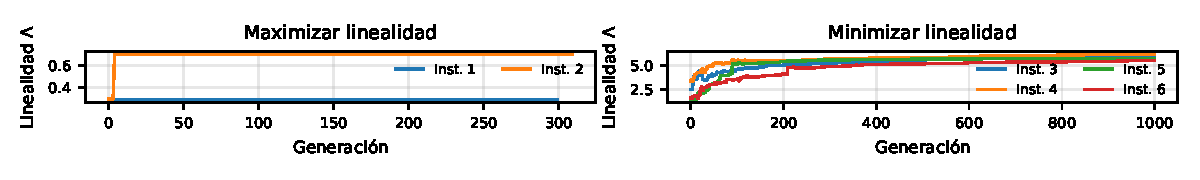
\includegraphics[width=\textwidth]{figuras/convergencia.pdf}
\caption{Linealidad $\Lambda$ del mejor nivel por generaci\'on (semilla 1).}\label{fig:conv}
\end{figure}

\begin{figure}[!htb]
\centering
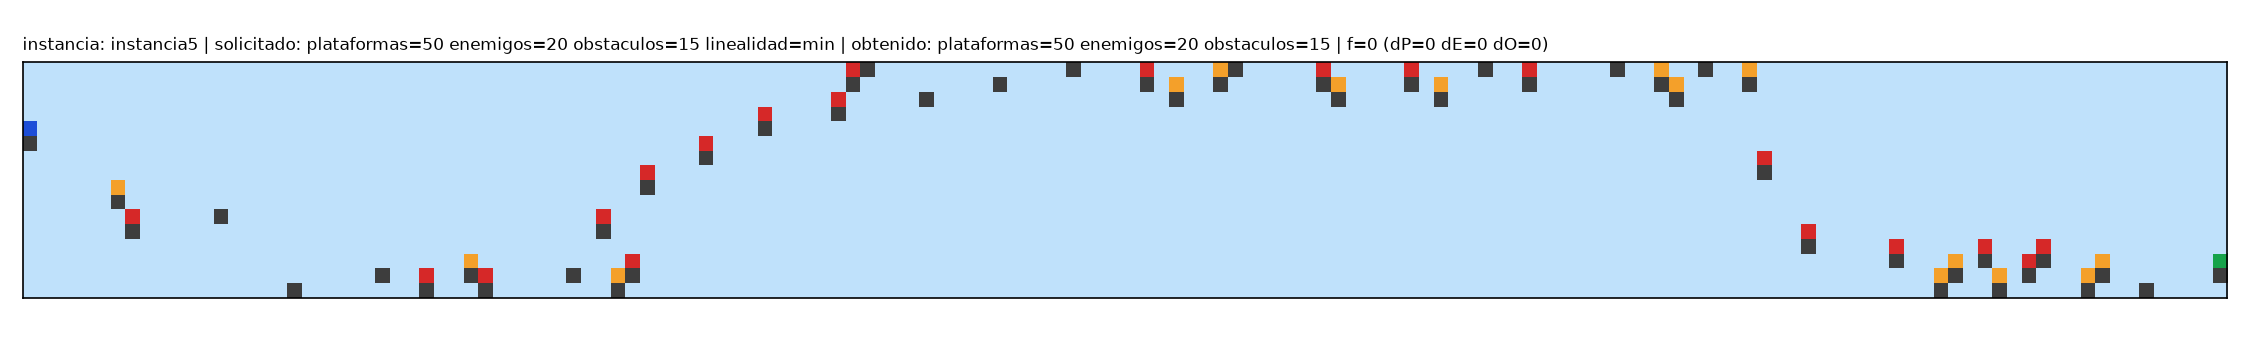
\includegraphics[width=.65\textwidth,trim=0 14 0 20,clip]{figuras/instancia5.png}
\caption{Nivel obtenido para la instancia 5 (minimizar linealidad, semilla 1). Azul: inicio; verde: meta; rojo: enemigos; naranjo: obst\'aculos.}\label{fig:niveles}
\end{figure}

\subsection{Variedad de los niveles}\label{sec:var}
Con 10 semillas por instancia (\texttt{experimentos/variedad.py}), las posiciones de las plataformas coinciden entre semillas en 51--57\% de las columnas y las alturas en 19--47\%. En las \emph{max}, los niveles usan entre 3,6 y 4,1 filas, casi rectos como corresponde a una linealidad alta, con una altura base distinta en cada semilla. En las \emph{min}, cada nivel usa las 16 filas, solo el 38--42\% de las plataformas est\'a en las dos filas m\'as usadas y el 100\% de los pares consecutivos cambia de altura. Una versi\'on previa, que solo minimizaba la desviaci\'on, usaba 6 filas, con 70--93\% de las plataformas en dos de ellas y la misma escalera entre un piso y un techo en todas las semillas; se corrigi\'o con $c$ y $r$. Persiste una limitaci\'on: la m\'etrica de regresi\'on sigue premiando las filas extremas, por lo que la forma de ``piso y techo'' es a\'un reconocible.

\subsection{Comparaci\'on con el estado del arte}
La comparaci\'on es cualitativa, pues cada trabajo usa otros juegos, agentes y hardware. El 100\% de niveles completables iguala a Launchpad, que lo garantiza por construcci\'on~\cite{Smith2011}, y supera el 87--100\% de FI-2Pop~\cite{Green2020} y el 97\% de las LSTM~\cite{Summerville2016}, aunque aqu\'i se mide con el modelo de salto y no con un agente. Las cantidades exactas se logran en 180 de 180 ejecuciones, mientras que Launchpad las controla solo en forma aproximada~\cite{Smith2011}, y el tiempo (0,3--2,5~s) es comparable al de PSO y GA~\cite{DePontes2022} (0,6--4~s).

%=============================================================================
\section{Conclusiones}\label{sec:conc}
%=============================================================================
La generaci\'on de niveles de plataformas es relevante para la PCG porque la validez de un nivel depende de relaciones finas entre sus elementos. Los m\'etodos constructivos, como Launchpad~\cite{Smith2011}, garantizan jugabilidad pero controlan poco el contenido; los basados en b\'usqueda~\cite{Dahlskog2013,DePontes2022} controlan el contenido pero no garantizan jugabilidad y su evaluaci\'on es dif\'icil de ajustar, y los basados en aprendizaje dependen de niveles de ejemplo~\cite{Summerville2016}. Ninguno busca cantidades exactas de elementos, la variante estudiada.

La propuesta combina una representaci\'on por columnas, que reduce el espacio de $10^{547}$ a $10^{251}$ niveles, un modelo de salto que discretiza la par\'abola en arreglos por distancia y un AE con movimientos dirigidos a las cantidades y por tramo para la forma del nivel. A diferencia de los m\'etodos de b\'usqueda revisados, que penalizan rasgos aislados~\cite{Dahlskog2013,DePontes2022} o recurren a un agente~\cite{Green2020}, el aporte principal es usar en la b\'usqueda un modelo f\'isico expl\'icito, similar al de los m\'etodos constructivos~\cite{Compton2006,Smith2011}, que verifica la completitud del nivel completo y permite evaluar entre 18.000 y 90.000 niveles por segundo.

Los resultados muestran que el AE obtiene niveles completables, sin plataformas inaccesibles y con $f=0$ en las 180 ejecuciones, en 1,1~s en promedio. Frente a la b\'usqueda aleatoria con el mismo presupuesto, empata en las instancias \emph{max}, que son f\'aciles, y es significativamente mejor en las \emph{min}, con niveles que cambian de altura en cada plataforma y usan las 16 filas, y entre 6 y 27 veces m\'as r\'apido. La mutaci\'on intermedia ($p_m=0{,}5$) dio los mejores resultados, y $L=50$ fue el tramo m\'as robusto.

Respecto de los supuestos, tratar la linealidad como criterio secundario mantuvo las cantidades exactas en todas las ejecuciones, pero la desviaci\'on respecto de la recta no captur\'o por s\'i sola los ``m\'ultiples cambios de altura'' de la baja linealidad~\cite{Saavedra2026}: al minimizarla, el AE la explotaba con mesetas en las filas extremas, por lo que se agregaron t\'erminos de variedad y de plataformas \'utiles a la funci\'on de evaluaci\'on, aunque a\'un se concentran en ellas. Como trabajo futuro, se propone medir la linealidad con los cambios de altura, validar la completitud con un agente~\cite{Green2020} y medir la variedad con el rango expresivo~\cite{Smith2011,Smith2010}.


%=============================================================================

\bibliographystyle{plain}
\bibliography{Referencias}

\subsection*{Declaraci\'on de uso de herramientas de IA}
\begingroup\small
\begin{enumerate}\setlength\itemsep{0pt}\setlength\parskip{0pt}
\item \textbf{Herramienta utilizada:} Claude Opus 5.5 (Anthropic) y Google Gemini (plan estudiante) en la Entrega 1; Claude Opus 5.5, Claude Sonnet 5.5 y Claude Code (todos de Anthropic) en la Entrega 2.
\item \textbf{Prop\'osito de uso:} En la Entrega 1, mejorar el entendimiento de los papers, construir un borrador inicial, revisar los avances en base a la r\'ubrica y mejorar la redacci\'on. En la Entrega 2, desarrollar el AE en paralelo con el estudiante, ayudar a aplicar los comentarios del ayudante en el modelo de salto y otros cambios, redactar el borrador, ayudar con el desarrollo de los experimentos y, finalmente, revisar el informe en base a las r\'ubricas y mejorar la redacci\'on.
\item \textbf{Prompts relevantes:} ``Necesito ayuda para entender X paper''; ``Ay\'udame a revisar este borrador en base a la r\'ubrica e instrucciones''; para la Entrega 2 se entreg\'o el contexto del proyecto a Claude para ayudar a construir el AE.
\item \textbf{Nivel de edici\'on:} La IA se utilizó para profundizar mejor el entendimiento de los conceptos y mejorar la redacci\'on del texto. Se le entregaron ideas y fue redactando un borrador que después fue revisado y modificado por el estudiante. Lo mismo se hizo en cuanto al funcionamiento del código a la hora de construir el algoritmo evolutivo. 
\item \textbf{Validaci\'on:} Papers del estado del arte, material del curso, compilaci\'on y ejecuci\'on del c\'odigo en las seis instancias y revisi\'on visual de los niveles generados.
\end{enumerate}
\endgroup

\end{document}
